\documentclass[onecolumn]{article}
%\usepackage{url}
%\usepackage{algorithmic}
\usepackage[a4paper]{geometry}
\usepackage{datetime}
\usepackage[margin=2em, font=small,labelfont=it]{caption}
\usepackage{graphicx}
\usepackage{mathpazo} % use palatino
\usepackage[scaled]{helvet} % helvetica
\usepackage{microtype}
\usepackage{amsmath}
\usepackage{subfigure}
\usepackage{float}

% Letterspacing macros
\newcommand{\spacecaps}[1]{\textls[200]{\MakeUppercase{#1}}}
\newcommand{\spacesc}[1]{\textls[50]{\textsc{\MakeLowercase{#1}}}}

\title{\spacecaps{Final Report: Skin Cancer: Malignant vs. Benign}\\ \normalsize \spacesc{CENG 3521, Data Mining} }

\author{Emre Ertürk, Ülkem Güleç\\emreerturk3@posta.mu.edu.tr, ulkemgulec@posta.mu.edu.tr}
%\date{\today\\\currenttime}
\date{\today}

\begin{document}
\maketitle

\begin{abstract}
Skin cancer is the out-of-control growth of abnormal cells in the epidermis, the outermost skin layer, caused by unrepaired DNA damage that triggers mutations. Cancer begins when healthy cells change and grow out of control, forming a mass called a tumor. A tumor can be cancerous or benign. A cancerous tumor is malignant, meaning it can grow and spread to other parts of the body. That report includes brief information on how to identify malignant and benign moles using image segmentation and image classification method



\end{abstract}

\section{Introduction}
Image segmentation is the process of partitioning an image into multiple different regions (or segments). The goal is to change the representation of the image into an easier and more meaningful image. We informed you about the skin cancer dataset in the first topic of our report. After that part, we have two main parts, one of them is image segmentation and another one is image classification. We mentioned clustering algorithms in the image segmentation part. Our report's last topic is about classifying segmented images.

\section{Skin Cancer Dataset}
This dataset contains a balanced dataset of images of benign skin moles and malignant skin moles. The malignant data has 1197 images and benign data has 1440 images. These images are 224x224 image dimensions.

\begin{figure}[H]
    \centering
    \subfloat
    \centering {{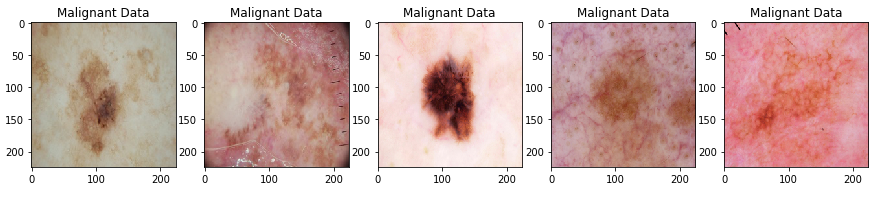
\includegraphics[width=15.0cm]{images/malignant5.png} }}%
    \qquad
    \subfloat
    \centering {{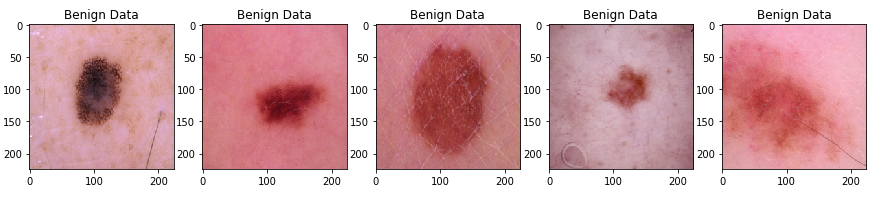
\includegraphics[width=15.0cm]{images/benign5.png} }}%
    \caption{Examples of malignant data and benign data}%
    \label{fig:2}%
\end{figure}


\section{Image Segmentation}
Image segmentation involves converting an image into a collection of regions of pixels that are represented by a mask or a labeled image.
By dividing an image into segments, you can process only the important segments of the image instead of processing the entire image. 

\subsection{k-means Clustering} % the star suppresses numbering of sections and subsections
K-means clustering is one of the popular unsupervised machine learning algorithms that groups objects into k groups based on their characteristics. The grouping is done minimizing the sum of the distances between each object and the group or cluster centroid.

\begin{figure}[H]
\centering
  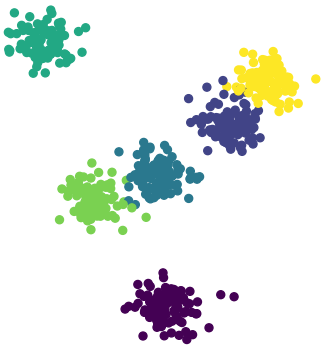
\includegraphics[scale=0.7]{images/cluster.png}
  \caption{Example of clustered data}
  \label{fig:4}
\end{figure}

\subsection{Elbow Algorithm} % the star suppresses numbering of sections and subsections
The Elbow method is a very popular technique and the idea is to run k-means clustering for a range of clusters k and for each value, we are calculating the sum of squared distances from each point to its assigned center. When the center are plotted and the plot looks like an arm then the “elbow” is the best value of k. In this project, we take an image to calculate the elbow number and as you can see in Figure 3. We found the best value of k as 2. So we assigned this number to the k\_cluster variable to use later.

\begin{figure}[H]
\centering
  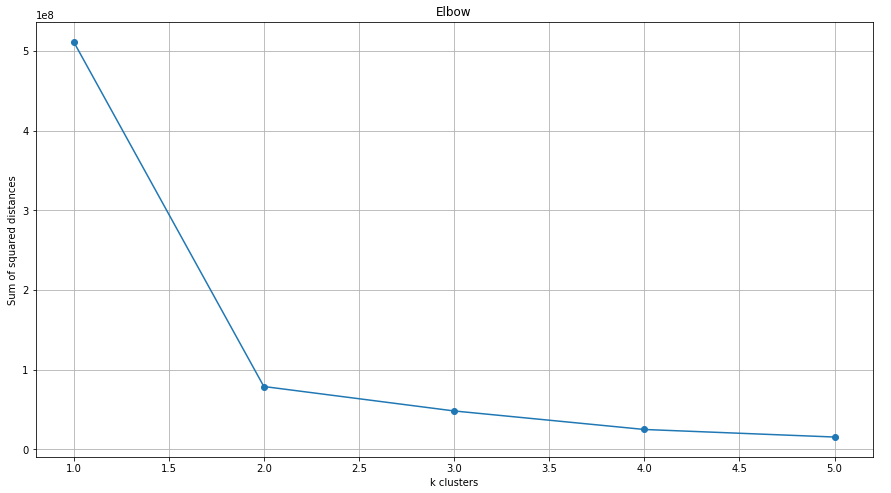
\includegraphics[scale=0.48]{images/elbow.PNG}
  \caption{Elbow Graph}
  \label{fig:4}
\end{figure}


\subsection{Color Processing}
We did some processes on images to put a mask. That mask helps us to classifying images.



\subsubsection{Rgb to Grey}
In this task firstly, we chose a malignant image. We converted this image into two colors using the rgb2grey() method. Then we gave this two-color image and optimal k\_clusters number as a parameter to the d2Kmeans function. Also, the d2Kmeans function is to calculate the k-means of a given image.

\begin{figure}[H]
\centering
  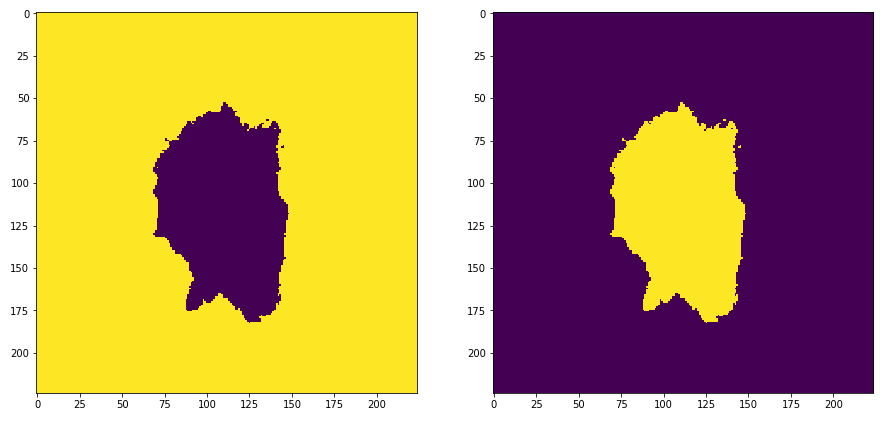
\includegraphics[scale=0.38]{images/rgb2grey.PNG}
  \caption{An image converted to two color}
  \label{fig:5}
\end{figure}

\subsubsection{Masked Image}
We applied the mask to an image. We used a mean filter algorithm to get a more smooth image. Then, we used the threshold\_otsu algorithm to get the binary image 

\begin{figure}[H]
\centering
  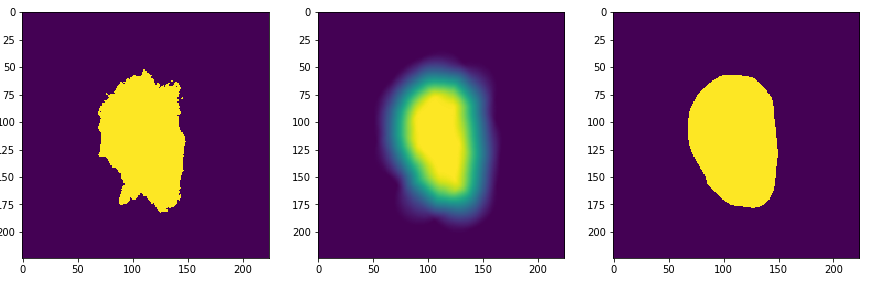
\includegraphics[scale=0.45]{images/median_filter, binary.png}
  \caption{The left one is the just grey image, the middle one is the median filtered image, the right one is the binary image
}
  \label{fig:5}
\end{figure}

We deleted the dark parts of the image. So we created a mask and we applied that mask to every image.

\begin{figure}[H]
\centering
  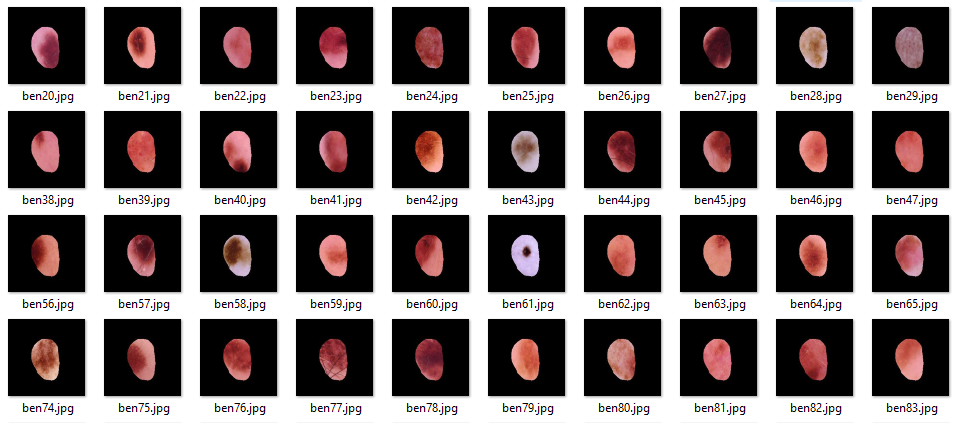
\includegraphics[scale=0.55]{images/masked.PNG}
  \caption{Masked images}
  \label{fig:5}
\end{figure}

\section{Image Classification}
Image classification is a supervised learning problem: define a set of target classes, and train a model to recognize them using labeled example photos.


\subsection{Hu Moments}
Firstly we converted image to grayscale using color.BGR2GRAY().
we used cv2.HuMoments() function to extract Hu Moments features from the image. The argument to this function is the moments of the image cv2.moments() flattened. It means we computed the moments of the image and convert it to a vector using flatten().

\begin{figure}[H]
\centering
  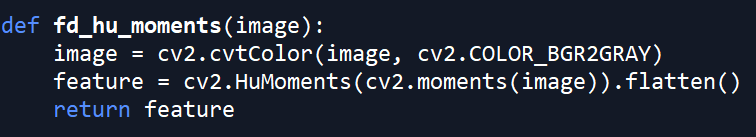
\includegraphics[scale=0.7]{images/fd_hu_moments.PNG}
  \caption{fd\_hu\_moments funtion}
  \label{fig:6}
\end{figure}


 
\subsection{Haralick Textures}
We converted our color image into a grayscale image as haralick feature descriptor expect images to be grayscale. We used mahotas.features.haralick() to extract Haralick Texture features from the image.


\begin{figure}[H]
\centering
  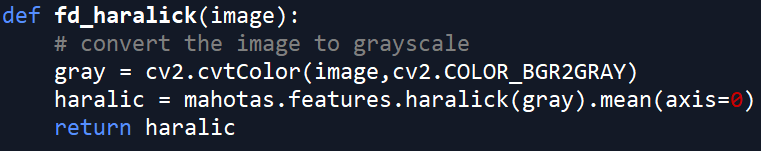
\includegraphics[scale=0.7]{images/fd_haralick.PNG}
  \caption{fd\_hu\_moments funtion}
  \label{fig:6}
\end{figure}


\subsection{Color Histogram}
We used the cv2.calcHist() function to extract Color Histogram features from the image. The arguments it expects are the image, channels, mask, histSize  and ranges for each channel (typically 0-256). Then we normalized the histogram using normalize() function of OpenCV and return a flattened version of this normalized matrix using flatten().


\begin{figure}[H]
\centering
  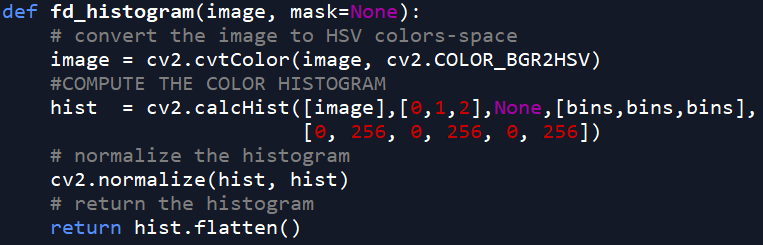
\includegraphics[scale=0.7]{images/fd_histogram.PNG}
  \caption{fd\_hu\_moments funtion}
  \label{fig:6}
\end{figure}

\subsection{Features of an image}
we extracted the three global features and concatenate these three features using NumPy’s np.hstack() function. These features came from color histogram, haralick textures and hu moments.

\begin{figure}[H]
\centering
  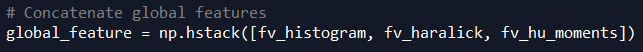
\includegraphics[scale=0.8]{images/global_feature.PNG}
  \caption{Concatenation of features}
  \label{fig:6}
\end{figure}

\subsection{Labels of our dataset}
We used LabelEncoder() method to encode our labels in a proper format. Our labels are 'mal' and 'ben', these are our subfolders name and types of moles.

\begin{figure}[H]
\centering
  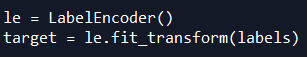
\includegraphics[scale=0.7]{images/labels.PNG}
  \caption{LabelEncoder()}
  \label{fig:6}
\end{figure}

\subsection{Training Data}
After all of these processes, we get proper data to use in classification methods. We compared seven different classification method using cross\_val\_score(). We observed the Random Forest Classifier method has the best accuracy score. .

\begin{figure}[H]
    \centering
    \subfloat
    \centering {{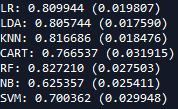
\includegraphics[width=5.0cm]{images/methods.PNG} }}%
    \qquad
    \subfloat
    \centering {{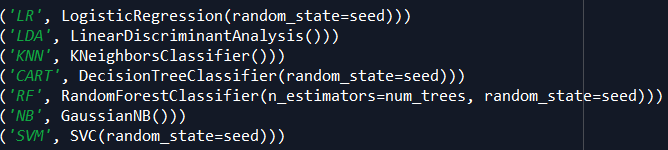
\includegraphics[width=15.0cm]{images/models2.PNG} }}%
    \caption{Comparisons of the seven classification}%
    \label{fig:2}%
\end{figure}

We split our data that randomly selected 70\% tuples are used for training while 30\% are used for testing. We applied our classification method and we fitted our train data to model. Then we calculated predictions using predict() method.
 
 \subsection{Test Data}
 At the end of the project we tested our algorithm using samples from segmented dataset. As you can see at the Figure 13 mostly results are okey but some results are wrong.
 
\begin{figure}[H]
    \centering
    \subfloat
    \centering {{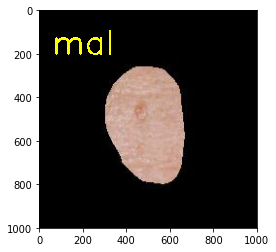
\includegraphics[width=5.0cm]{images/mal1.png} }}%
    \qquad
    \subfloat
    \centering {{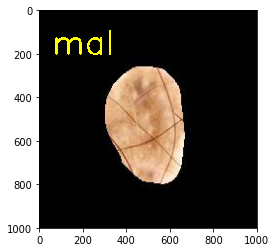
\includegraphics[width=5.0cm]{images/mal2.png} }}%
    \qquad
    \subfloat
    \centering {{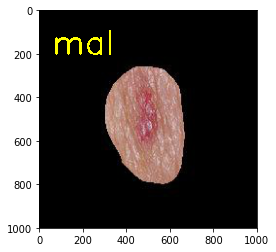
\includegraphics[width=5.0cm]{images/mal3.png} }}%
    \qquad
    \subfloat
    \centering {{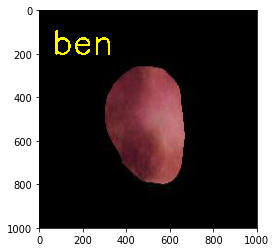
\includegraphics[width=5.0cm]{images/mal4.png} }}%
    \qquad
    \subfloat
    \centering {{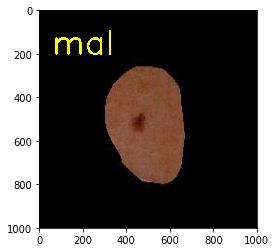
\includegraphics[width=5.0cm]{images/mal5.png} }}%
    \qquad
    \subfloat
    \centering {{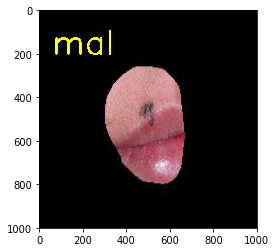
\includegraphics[width=5.0cm]{images/mal6.png} }}%
    \caption{These images taken from the malignant dataset}%
    \label{fig:2}%
\end{figure}

\section{Conclusion}
In conclusion, image segmentation methods help us to get better classifying results. We used the clustering method in the image segmentation part. After the segmentation part, we decided which classification method is the most proper for our dataset. We compared seven different classification methods using a cross-validation score. Before doing that, we converted data to readable for classification methods. As a result, we learned the image segmentation and classifying algorithms.




\nocite{*}
\bibliographystyle{plain}
\bibliography{references}
\end{document}

